\section{Shape reconstruction}

\begin{theorem}
    A projective transformation $\mathbf{H}$ that maps the circular points $\mathbf{I}$ and $\mathbf{J}$ onto themselves implies that $\mathbf{H}$ is a similarity transformation.
\end{theorem}
\begin{proof}
    When a similarity transformation matrix $\mathbf{H}_\text{S}$ is applied to the circular point $\mathbf{I}$, it produces a scalar multiple of $\mathbf{I}$.
    The same holds true for the other circular point, $\mathbf{J}$.
    Since both $\mathbf{I}$ and $\mathbf{J}$ remain unchanged under this transformation, $\mathbf{H}_\text{S}$ is indeed a similarity transformation.
\end{proof}
In a general projective mapping of the original scene, the images of the circular points, denoted as $(\mathbf{I}^\prime,\mathbf{J}^\prime)$, do not coincide with the original circular points $\mathbf{I}$ and $\mathbf{J}$. 
To perform shape reconstruction, we apply a corrective projective transformation $\mathbf{H}_\text{SR}$ that maps $\mathbf{I}^\prime$ and $\mathbf{J}^\prime$ back to $\mathbf{I}$ and $\mathbf{J}$, respectively. 
This results in a modified image where the circular points are restored to their original positions.

According to the theorem, this new transformation results in a similarity transformation of the original scene. 
Hence, the reconstructed model is a shape reconstruction, maintaining the overall proportions and geometry of the original scene.
\begin{figure}[H]
    \centering
    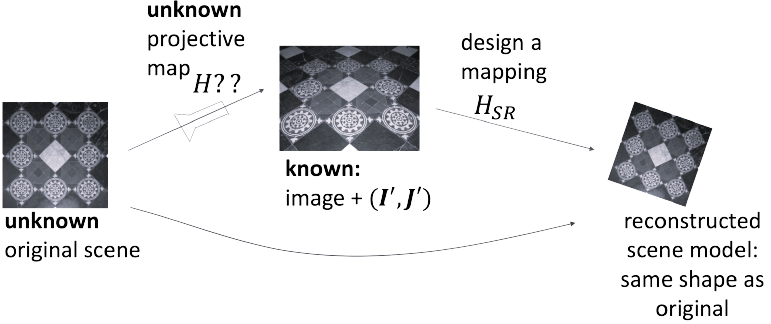
\includegraphics[width=0.75\linewidth]{images/HSR.png}
\end{figure}
The main challenges in this approach are:
\begin{itemize}
    \item Finding the projective transformation $\mathbf{H}_\text{SR}$ that restores the points $\mathbf{I}^\prime$ and $\mathbf{J}^\prime$ to $\mathbf{I}$ and $\mathbf{J}$. 
    \item Determining the vanishing line in the image to aid in finding the circular points.
\end{itemize}

\subsection{Projective transformation determination}
Finding the projective transformation $\mathbf{H}_\text{SR}$ that maps $\mathbf{I}^\prime$ and $\mathbf{J}^\prime$ back to $\mathbf{I}$ and $\mathbf{J}$ is equivalent to solving for one of the infinitely many matrices that satisfy:
\[\begin{cases}
    \mathbf{H}_\text{SR}\mathbf{I}^\prime=\mathbf{I} \\
    \mathbf{H}_\text{SR}\mathbf{J}^\prime=\mathbf{J}
\end{cases}\]
This task is non-trivial, but it can be simplified by leveraging additional geometric information, such as the degenerate conic dual to the circular points.

The degenerate conic dual to $\mathbf{I}^\prime,\mathbf{J}^\prime$ is given by:
\[\mathbf{C}_{\infty}^{\prime\ast}=\mathbf{I}^\prime \mathbf{J}^{\prime T}+\mathbf{J}^\prime \mathbf{I}^{\prime T}\]
This conic is the image of the original conic dual to the circular points $\mathbf{I}$ and $\mathbf{IJ}$, denoted by:
\[\mathbf{C}_{\infty}^\ast=\mathbf{IJ}^{T}+\mathbf{JI}^{T}\]
Since $\mathbf{C}_{\infty}^{\prime\ast}$ is the projective image of $\mathbf{C}_\infty^\ast$, any projective transformation $\mathbf{H}_\text{SR}$ that restores $\mathbf{I}^\prime$ and $\mathbf{J}^\prime$ to $\mathbf{I}$ and $\mathbf{J}$ will also restore $\mathbf{C}_{\infty}^{\prime\ast}$ to $\mathbf{C}_{\infty}^\ast$. 
Using the transformation rule for dual conics, we have:
\[\mathbf{C}^\ast_{\infty}=\mathbf{H}_\text{SR}\mathbf{C}^{\prime\ast}_{\infty}\mathbf{H}_\text{SR}^T\]
Reversing this relationship gives:
\[\mathbf{C}_{\infty}^{\prime\ast}=\mathbf{H}_\text{SR}^{-1} \begin{bmatrix} 1 & 0 & 0 \\ 0 & 1 & 0 \\ 0 & 0 & 0 \end{bmatrix} \mathbf{H}_\text{SR}^{-T}\]

By applying singular value decomposition (SVD) to the equation above, we find that $\mathbf{H}_\text{SR}^{-1}$ and $\mathbf{H}_\text{SR}^{-T}$ are orthogonal matrices. 
This leads to: 
\[\text{SVD}\left(\mathbf{C}_{\infty}^{\prime\ast}\right)=\mathbf{U}_\perp \begin{bmatrix} 1 & 0 & 0 \\ 0 & 1 & 0 \\ 0 & 0 & 0 \end{bmatrix} \mathbf{U}_{\perp}^T\]
Thus, the solution for $\mathbf{H}_\text{SR}$ is:
\[\mathbf{H}_\text{SR} = \mathbf{U}_{\perp}^{-1}=\mathbf{U}_{\perp}^T\]
To ensure proper image rectification and scaling, the matrix $\mathbf{H}_\text{SR}$ can be adjusted to:
\[\mathbf{H}_\text{SR} = \begin{bmatrix} \frac{1}{\sqrt{a}} & 0 & 0 \\ 0 & \frac{1}{\sqrt{b}} & 0 \\ 0 & 0 & 1 \end{bmatrix} \mathbf{U}^T\]
This transformation not only maps the circular points back to their original positions but also ensures that the final image is a faithful similarity reconstruction of the scene.

































\subsection{Vanishing line identification}
To determine the vanishing line, one can leverage additional information from the observed scene. 
This information can be used to establish the following constraints:
\begin{enumerate}
    \item Known angles between lines: when the angles between lines in the scene are known, these angles can be used to constrain the vanishing line. 
        The angle between two lines is related to the angle between their normal directions and is independent of parameters $c_1$ and $c_2$. 
        Mathematically, this relationship is expressed as:
        \[\cos\vartheta=\dfrac{a_1a_2+b_1b_2}{\sqrt{(a_1^2+b_1^2)(a_2^2+b_2^2)}}\]
        Here, $a_1$, $b_1$, $a_2$, and $b_2$ are coefficients of the normal vectors of the lines. 
        By rewriting the terms, this equation can be expressed as: 
        \[\cos\vartheta=\dfrac{l^TC_{\infty}^\ast m}{\sqrt{(l^TC_{\infty}^\ast l)(m^TC_{\infty}^\ast m)}}\]
        This equation can be further simplified by using the rules obtaining $C_{\infty}^\ast=H^{-1}C_{\infty}^{*'}H^{-T}$.  
        Now, we can rewrite $l^TC_{\infty}^\ast m$ as $l^{\prime T}C_{\infty}^{*'}m^\prime$. 
        With these transformations, the equation becomes:
        \[\cos\vartheta=\dfrac{l^{\prime T}C_{\infty}^{*'}m^\prime}{(l^{\prime T}C_{\infty}^{*'}l^\prime)(m^{\prime T}C_{\infty}^{*'}m^\prime)}\]
        In this case, $m^\prime$ and $l^\prime$ are obtained from the image. 
        Since the angle is known, this equation provides a linear constraint on $C_{\infty}^{*'}$, that is linear when the lines are perpendicular ($\cos\vartheta=0$).
        The unknown matrix $C_{\infty}^\prime$ is symmetric, homogeneous, and singular, providing four independent constraints.
    \item Known shape of objects: if the shape of objects in the scene is known, the reconstruction matrix $\mathbf{H}_\text{SR}$ can be determined. 
        The transformation matrix is defined as:
        \[\mathbf{H}_\text{SR}=
        \begin{bmatrix}
            \frac{1}{\sqrt{a}} & 0 & 0 \\
            0 & \frac{1}{\sqrt{b}} & 0 \\
            0 & 0 & 1
        \end{bmatrix}
        U^T
        \]
        The Euclidean reconstructed image is calculated as $M_S=\mathbf{H}_\text{SR} \cdot \textnormal{image}$
    \item Combinations of constraints: it is also possible to use a combination of known angles between lines and the shape of objects for additional constraints.
    \item Observation of rigid planar motion: when observing rigid planar motion, which is a similarity transformation, the circular points remain invariant.
        The object has three degrees of freedom, and the center of rotation and the rotation angle can be determined.
        Given a matrix $H$, the eigenvectors of $H$ correspond to fixed points, and the eigenvectors of $H^{-T}$ correspond to fixed lines of the transformation.
        The eigenvectors can be used to extract important information:
        \begin{itemize}
            \item Eigenvectors $\mathbf{I}^\prime,\mathbf{J}^\prime$ correspond to complex eigenvalues. 
            \item The phase of these eigenvectors is the rotation angle.
            \item Eigenvector $O^\prime$ correspond to real eigenvalues. 
        \end{itemize}
        The three eigenvectors of $H$ are proportional to three distinct values: 1, $e^{i\theta}$, and $-e^{i\theta}$.
        The eigenvector corresponding to the eigenvalue 1 represents the image of the center of rotation, denoted as $O$, and the angle $\theta$ corresponds to the rotation angle. 
        The eigenvectors associated with the complex eigenvalues represent the images of the circular points $\mathbf{I}^\prime,\mathbf{J}^\prime$. 
        Therefore, using the relationship $C_{\infty}^{\prime\ast}=\mathbf{I}^\prime J^{\prime T}+\mathbf{J}^\prime I^{\prime T}$, the singular value decomposition can be applied to obtain $\text{SVD}(C_{\infty}^{\prime\ast})=UC_{\infty}^\ast U^T$, where $U^T$ is the rectification matrix. 
        Two methods can be used to address this:
        \begin{itemize}
            \item Direct method: 
                \begin{enumerate}
                    \item Find $C_{\infty}^{*'}$. 
                    \item Compute $H_{rect}$ for rectification. 
                \end{enumerate}
            \item Stratified method: 
                \begin{enumerate}
                    \item Perform affine reconstruction from projective to affine.
                    \item Perform shape reconstruction from affine to metric.
                \end{enumerate}
        \end{itemize}
        In some cases, the stratified method reduces numerical errors, providing a more accurate result.
\end{enumerate}